\documentclass[border=10pt]{standalone}
\usepackage{pgfplots}
\pgfplotsset{compat=1.18}
\begin{document}
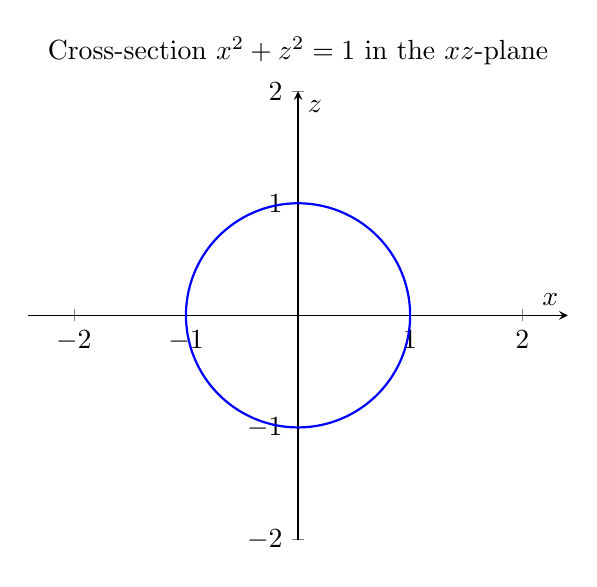
\begin{tikzpicture}
\begin{axis}[
    axis equal,
    axis lines=center,
    xlabel={$x$}, ylabel={$z$},
    xmin=-2, xmax=2, ymin=-2, ymax=2,
    title={Cross-section $x^2+z^2=1$ in the $xz$-plane}
]
\addplot[blue, thick, domain=0:360, samples=200, variable=\t]
({cos(t)}, {sin(t)});
\end{axis}
\end{tikzpicture}
\end{document}
